% !TeX root = Slides-Chapter01.tex
%!TEX TS-program = Arara
% arara: pdflatex: {shell: yes}
% arara: pdflatex: {shell: yes}
% arara: clean: { extensions: [ log, aux, nav, out, snm, vrb, toc, gz ] }


\section{A section, like a chapter}

\begin{frame}
\frametitle{Some basic itemize}
\framesubtitle{Some Subtitle}

\begin{itemize}
\item A bullet point  \okay
\item A bullet point  
\item A bullet point  
\item A bullet point  
\item A bullet point  
\end{itemize}
\end{frame}



\begin{frame}
\frametitle{An Image}
\framesubtitle{~}

\begin{center}
\begin{figure}
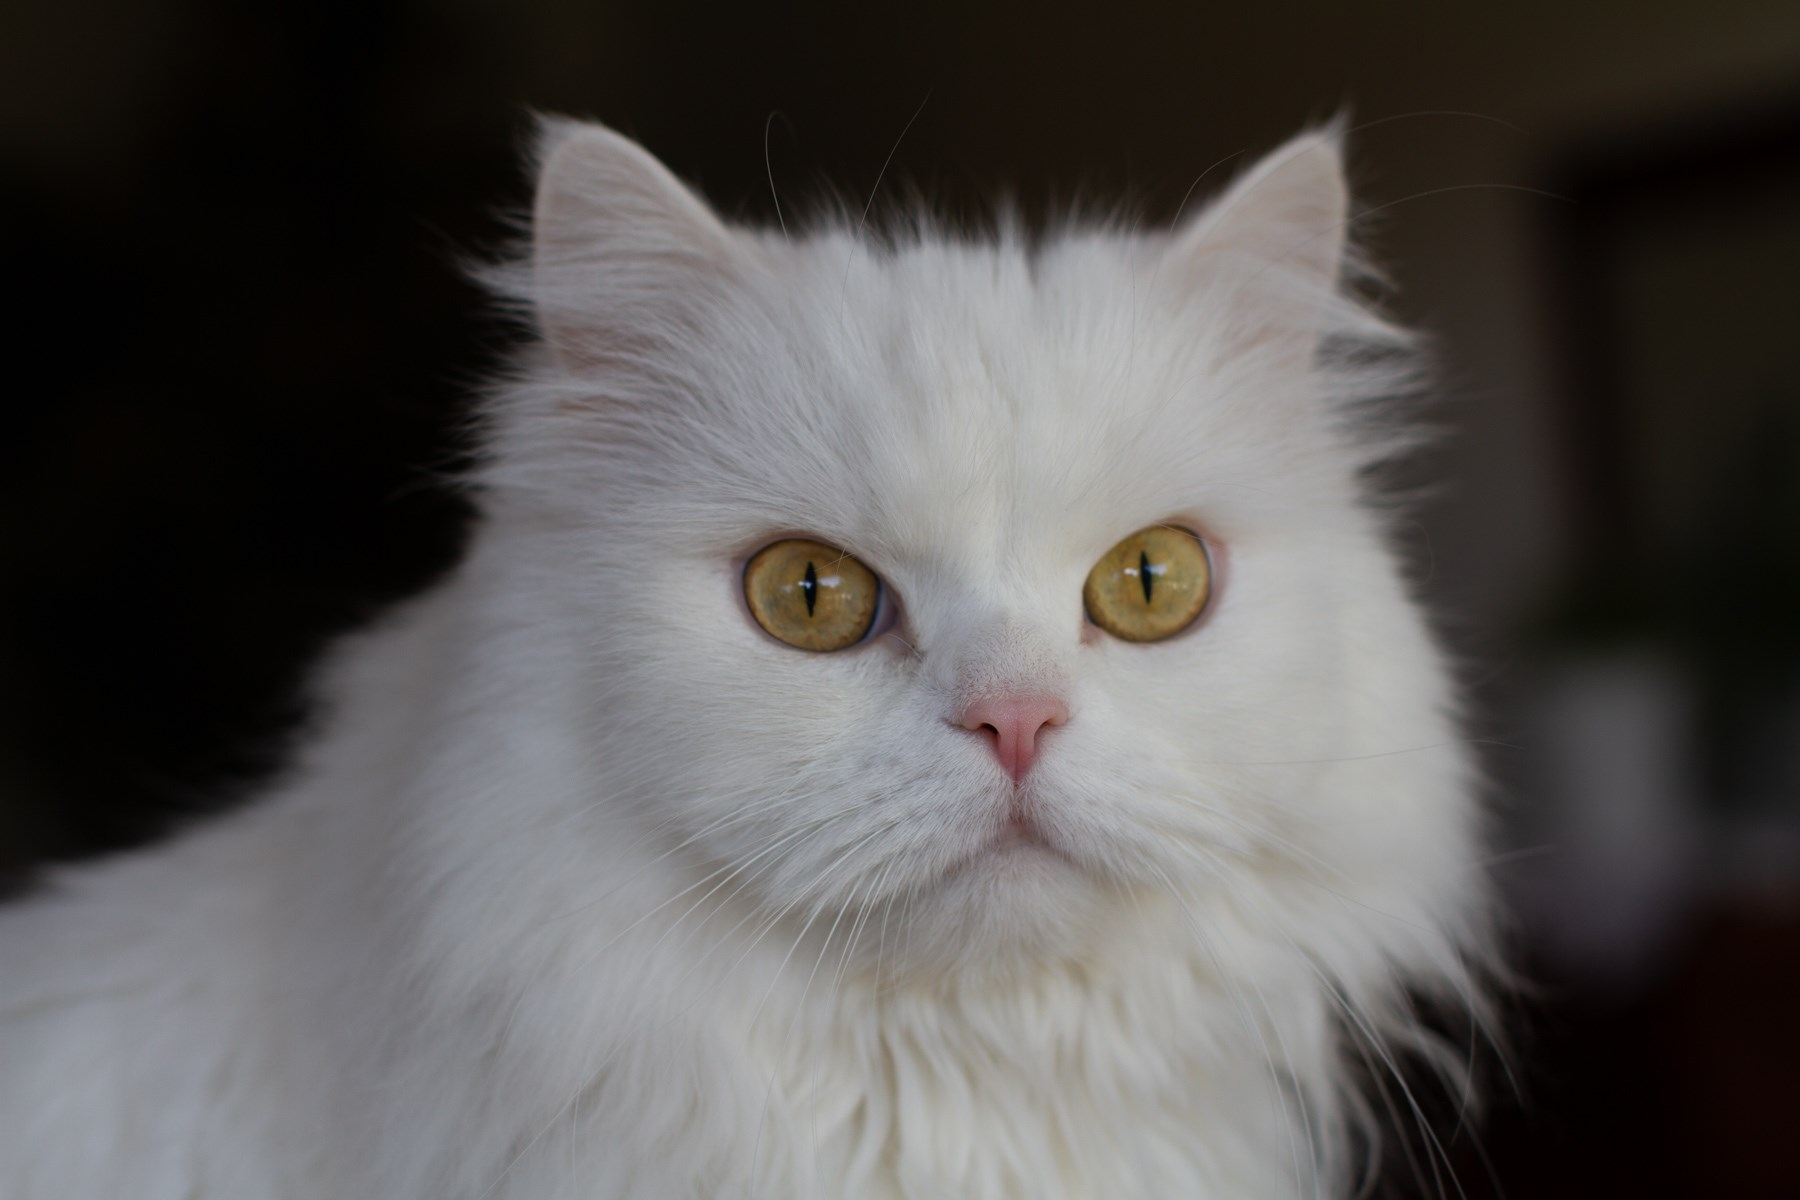
\includegraphics[width=0.9\textwidth]{Images/testimage}
\caption{This is a cat}\label{fig:cat}
\end{figure}
\end{center}

\end{frame}


\begin{frame}
\frametitle{An Image}
\framesubtitle{\textbackslash bilds\{<image>\}}

\bilds{Images/testimage}

\end{frame}


\begin{frame}
\frametitle{An Image}
\framesubtitle{\textbackslash bild\{<scale>\}\{<image>\}\{<caption>\}}

\bild{0.8}{Images/testimage}{The Caption}

\end{frame}


\begin{frame}
\frametitle{An Image}
\framesubtitle{\textbackslash bildf\{<scale>\}\{<image>\}\{<caption>\}}

\bildf{0.8}{Images/testimage}{The Caption}

\end{frame}


\begin{frame}
\frametitle{An Image}
\framesubtitle{\textbackslash bildfc\{<scale>\}\{<image>\}\{<caption>\}}

\bildfc{0.4}{Images/testimage}{The Caption}

\end{frame}



\begin{frame}
\frametitle{Some basic Math}
\framesubtitle{~}

\begin{equation}
x_{1,2} = - \frac{p}{2} \pm 
\sqrt{ 
	\left( 
		\frac{p}{2} 
	\right)^2 
	- q}
\end{equation}

\end{frame}


\begin{frame}[fragile]
\frametitle{Some Code Listing}
\framesubtitle{Manual lstlisting env}

\begin{lstlisting}[language={Python}, caption={A square class in Python}, label={lis:square}]
class Square():

    def __init__(self, sidelength = 1):
        self.length = sidelength
        
    def calculate_circumference(self):
        return 4 * self.length
        
    def calculate_area(self):
        return self.length**2

q = Square(sidelength=25)
print(q.calculate_circumference())
print(q.calculate_area())
\end{lstlisting}

\end{frame}



\begin{frame}[fragile]
\frametitle{Some Code Listing}
\framesubtitle{Manual lstinputlisting}

\lstinputlisting[language={Python}, caption={Another square class in Python}, label={lis:square}]{Listings/Square.py}

\end{frame}


\begin{frame}[fragile]
\frametitle{Some Code Listing}
\framesubtitle{\textbackslash pypy\{Caption\}\{File\}}

\pypy{The Caption}{Listings/Square.py}


\end{frame}






